\section{Tagging}
The tagging part of the system is one of the primary pillars of the system. The implementation of the concept consists of multiple parts, such as creating and maintaining the tags, attaching tags to assets, searching for tags through assets, etc.
\par
Most of these parts have not been included in this section, because they are easily implemented and/or trivial. The parts chosen for this section are the handling of users, connections between multiple tags, connections to departments, and the attachment of tags to assets and the effects of this.

\subsection{Users as tags}
To make it possible to attach users to assets, they implement the \textit{ITagable} interface. This interface is set as the type of all lists containing tags and users, and by creating an abstraction they both implement, it is possible to avoid specifically addressing tags or users. The interface demands the implementing classes to contain all the attributes related to an asset. This makes it possible to handle users and tags the same way in situations such as attaching users and tags to an asset or searching the assets based on attached users and tags.

\subsection{Parent-child and department relation}
To better organize tags, each tag can belong to a department. This will decrease the number of tags being shown in the suggestions across the application and will make it easier for the user to find the right tag. If a tag is universal, such as the user tag, the department of the tag is set to \textit{All Departments}, in which case they will appear no matter the current department of the user.
\par
The separation of the tags into departments improves the overall simplicity of the system, but a single department can still end up containing a large amount of tags. To further divide the amount of tags, and ease the task of finding the right tag, a hierarchical structure has been added through parent tags.
\par
Every tag belongs to a department, possibly \textit{All Departments}, but by the introduction of parent tags, they can also belong to another tag. This way, fields, color, and department of a tag can be inherited by other tags. This also makes it easier to create a number of tags with the same fields.
\par
The hierarchic structure of the tags and departments only has three levels, as a parent tag cannot belong to another parent tag (see \autoref{fig:TagHierarchicStructureWithDepartment}).

\begin{figure}[H]
    \centering
    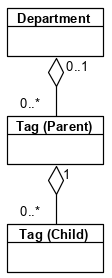
\includegraphics[width=0.18\textwidth]{figures/Implementation/TagHierarchicStructure.png}
    \caption{The hierarchic structure of the parent-child relation of tags}
    \label{fig:TagHierarchicStructureWithDepartment}
\end{figure}

In this implementation, a tag is by default a parent tag without any children. A child tag is created by setting the parent tag of the tag. This means that a parent tag can have no children, but a child tag must have a parent, otherwise it will be a parent itself.
\par
The connection between the parent and its children is an aggregation, as the children will inherit the fields, color, and department of the parent. The color can then be changed to something different, but the department is locked in place, as accessing children belonging to another department than their parent should not be possible, because the user has to go through the parent to access the children.
\par
Within the system, the parents and children are treated different in a few situations. One of these situations is when searching through assets. When searching for an asset in the \textit{AssetList}, trying to apply a parent tag with children will enter the parent tag and let the user add its children to the search. If the parent tag has no children, it is added to the search. This distinction between children and parents make it possible to suggest a smaller number of tags at a time, and still letting the user access all tags in the current department.

\subsection{Asset-tag relation}
Attaching tags to assets is the main purpose of the tags. When a tag is attached to an asset, the asset inherits the fields from the tag and an instance of the \textit{Asset-tag relation} class (see \autoref{fig:ModelComponentClassDiagram}) would be generated. This class, however, has not been implemented in the system but exists in the database as two relational tables, one for the relation between the asset and tag tables and one for the relation between the asset and user tables. For simplicity, only the table connecting the asset and tag tables have been described, but the same principles apply to the relation between the asset and user tables. The reason for having two different tables is that a tag and a user can both have the same database ID, which could cause issues if they were placed in the same table.
\par
A row in the relational table contains an ID and the IDs of an asset and a tag. When fetching either assets or tags, the table can be used to get all the objects of one connected to a specific instance of the other. This relational table also makes it possible to have a single tag attached to multiple assets, without copying the tag to every asset and keeping the relational table up to date, even if either the tag or the asset is updated.
\\
This relational table also ensures that additional fields added to a tag can be added to the assets with the given tag when they are opened for editing. The fields could be added as soon as the tag is updated, but if the tag is attached to hundreds of assets, the value of the field would potentially have to be set for all these assets.
\par
Adding or removing a tag from an asset is as simple as adding or removing a row in the relational table. If the assets were connected to tags directly, the removal of a tag would demand every asset connected to the tag to be updated, which would be a resource intensive operation.
\par
The relational table also makes it possible to search for assets based on the tags attached to them, as mentioned above. This makes it easier to find assets and gives the opportunity to filter the assets based on attached users and tags.
\par
The primary advantage of using a relational table is that the data will only exist once throughout the database and updating an entry will only have to be done once. The biggest problem of the relational table is its increase to run time as the database grows. The increase in execution time is caused by the fact that the table must be iterated through to find the correct relation. This however has been improved by using an index, which maps the search to the table, which removes the need to iterate through every entry \citep{RelationalTable}.
\par
% The method takes in a list of tag IDs. The \textit{asset\_tags} table is used to find the IDs of assets with a connection to one of the tag IDs. This list is then used to fetch a list of assets from the \textit{assets} table in the database. Lastly, the assets are returned as a list to call place.
% \par
A good example of the use of the relational tables is the method in \textit{AssetRepository} that attaches tags and users to an asset (see \autoref{code:AssetRepositoryAttachTags}). This method takes in an asset and a list of \textit{ITagable}'s. This way, the method can simply be called once and all the asset-tag and asset-user relations are created. Because the tags and users are in two different tables, and both could be in the input list, the method has to check which table each connection should be placed in, and inserts it. 
\par
Lines 11 - 14 in \autoref{code:AssetRepositoryAttachTags} creates a list of \textit{Users} and \textit{Tags} from the single list of \textit{ITagable}'s.
Then an SQL query, specifying that the following values should be inserted into the asset\_users table, is created. Then in lines 20 - 26 is a for-loop that iterates over the list of \textit{Users}, adding the id's of the users and the assets to the query. \par
The same process is repeated for the list of \textit{Tags} in lines 30 - 36, where the id's are inserted into the asset\_tags table.

\begin{listing}[H]
\begin{minted}[frame=lines, framesep=3mm, baselinestretch=1, linenos, bgcolor=LightGray, escapeinside='', breaklines]{csharp}
public bool AttachTags(Asset asset, List<ITagable> listOfTags)
{
    ...
        
    List<User> users = listOfTags.OfType<User>().ToList();
    List<Tag> tags = listOfTags.OfType<Tag>().ToList();
    int userCounter = users.Count;
    int tagCounter = tags.Count;
        
       ...

            StringBuilder userQuery = new StringBuilder("INSERT INTO asset_users VALUES ");

            for (int i = 0; i < userCounter; i++)
            {
                userQuery.AppendFormat("({0},{1})", asset.ID, users[i].ID);

                if (i != userCounter - 1)
                    userQuery.Append(",");
            }

            StringBuilder tagQuery = new StringBuilder("INSERT INTO asset_tags VALUES ");

            for (int i = 0; i < tagCounter; i++)
            {
                tagQuery.AppendFormat("({0},{1})", asset.ID, tags[i].ID);
                
                if (i != tagCounter - 1)
                    tagQuery.Append(",");
            }
            
           ...
    return querySuccess;
}
\end{minted}
\captionof{listing}{AssetRepository AttachTags method}
\label{code:AssetRepositoryAttachTags}
\end{listing}
\todo[inline]{Indsæt igen, når Exceptions bliver håndteret}